\documentclass{article}
\usepackage{iclr2027_conference,times}
\usepackage{hyperref}
\usepackage{url}
\usepackage{graphicx}
\usepackage{booktabs}
\usepackage{amsmath}
\usepackage{xcolor}
\graphicspath{{figs/}}
\newcommand{\eacMiniNone}{2/100}
\newcommand{\eacPctMiniNone}{2}
\newcommand{\eacCIMiniNone}{[1,7]}
\newcommand{\execMiniNone}{5/50}
\newcommand{\execPctMiniNone}{10}
\newcommand{\ctrlMiniNone}{3/50}
\newcommand{\ctrlPctMiniNone}{6}
\newcommand{\noticeMiniNone}{50}
\newcommand{\execSeenMiniNone}{20}
\newcommand{\tokMiniNone}{21}
\newcommand{\choresMiniNone}{3.5}
\newcommand{\eacMiniBank}{56/100}
\newcommand{\eacPctMiniBank}{56}
\newcommand{\eacCIMiniBank}{[46,65]}
\newcommand{\execMiniBank}{28/50}
\newcommand{\execPctMiniBank}{56}
\newcommand{\ctrlMiniBank}{4/50}
\newcommand{\ctrlPctMiniBank}{8}
\newcommand{\noticeMiniBank}{70}
\newcommand{\execSeenMiniBank}{80}
\newcommand{\tokMiniBank}{54}
\newcommand{\choresMiniBank}{7.4}
\newcommand{\eacMiniSchedone}{42/100}
\newcommand{\eacPctMiniSchedone}{42}
\newcommand{\eacCIMiniSchedone}{[33,52]}
\newcommand{\execMiniSchedone}{43/50}
\newcommand{\execPctMiniSchedone}{86}
\newcommand{\ctrlMiniSchedone}{4/50}
\newcommand{\ctrlPctMiniSchedone}{8}
\newcommand{\noticeMiniSchedone}{86}
\newcommand{\execSeenMiniSchedone}{100}
\newcommand{\tokMiniSchedone}{18}
\newcommand{\choresMiniSchedone}{2.2}
\newcommand{\eacMiniSched}{6/100}
\newcommand{\eacPctMiniSched}{6}
\newcommand{\eacCIMiniSched}{[3,12]}
\newcommand{\execMiniSched}{46/50}
\newcommand{\execPctMiniSched}{92}
\newcommand{\ctrlMiniSched}{2/50}
\newcommand{\ctrlPctMiniSched}{4}
\newcommand{\noticeMiniSched}{92}
\newcommand{\execSeenMiniSched}{100}
\newcommand{\tokMiniSched}{18}
\newcommand{\choresMiniSched}{2.2}
\newcommand{\eacMiniSchedtwo}{7/100}
\newcommand{\eacPctMiniSchedtwo}{7}
\newcommand{\eacCIMiniSchedtwo}{[3,14]}
\newcommand{\execMiniSchedtwo}{35/50}
\newcommand{\execPctMiniSchedtwo}{70}
\newcommand{\ctrlMiniSchedtwo}{2/50}
\newcommand{\ctrlPctMiniSchedtwo}{4}
\newcommand{\noticeMiniSchedtwo}{74}
\newcommand{\execSeenMiniSchedtwo}{95}
\newcommand{\tokMiniSchedtwo}{56}
\newcommand{\choresMiniSchedtwo}{7.7}
\newcommand{\eacMiniRwim}{5/40}
\newcommand{\eacPctMiniRwim}{12}
\newcommand{\eacCIMiniRwim}{[5,26]}
\newcommand{\execMiniRwim}{2/20}
\newcommand{\execPctMiniRwim}{10}
\newcommand{\ctrlMiniRwim}{1/20}
\newcommand{\ctrlPctMiniRwim}{5}
\newcommand{\noticeMiniRwim}{70}
\newcommand{\execSeenMiniRwim}{14}
\newcommand{\tokMiniRwim}{78}
\newcommand{\choresMiniRwim}{7.7}
\newcommand{\eacDeepseekNone}{1/100}
\newcommand{\eacPctDeepseekNone}{1}
\newcommand{\eacCIDeepseekNone}{[0,5]}
\newcommand{\execDeepseekNone}{1/50}
\newcommand{\execPctDeepseekNone}{2}
\newcommand{\ctrlDeepseekNone}{1/50}
\newcommand{\ctrlPctDeepseekNone}{2}
\newcommand{\noticeDeepseekNone}{30}
\newcommand{\execSeenDeepseekNone}{7}
\newcommand{\tokDeepseekNone}{8}
\newcommand{\choresDeepseekNone}{1.6}
\newcommand{\eacDeepseekBank}{64/100}
\newcommand{\eacPctDeepseekBank}{64}
\newcommand{\eacCIDeepseekBank}{[54,73]}
\newcommand{\execDeepseekBank}{34/50}
\newcommand{\execPctDeepseekBank}{68}
\newcommand{\ctrlDeepseekBank}{3/50}
\newcommand{\ctrlPctDeepseekBank}{6}
\newcommand{\noticeDeepseekBank}{78}
\newcommand{\execSeenDeepseekBank}{87}
\newcommand{\tokDeepseekBank}{53}
\newcommand{\choresDeepseekBank}{7.7}
\newcommand{\eacDeepseekSched}{0/49}
\newcommand{\eacPctDeepseekSched}{0}
\newcommand{\eacCIDeepseekSched}{[0,7]}
\newcommand{\execDeepseekSched}{18/49}
\newcommand{\execPctDeepseekSched}{37}
\newcommand{\ctrlDeepseekSched}{0/49}
\newcommand{\ctrlPctDeepseekSched}{0}
\newcommand{\noticeDeepseekSched}{45}
\newcommand{\execSeenDeepseekSched}{82}
\newcommand{\tokDeepseekSched}{10}
\newcommand{\choresDeepseekSched}{1.7}
\newcommand{\eacDeepseekSchedtwo}{3/100}
\newcommand{\eacPctDeepseekSchedtwo}{3}
\newcommand{\eacCIDeepseekSchedtwo}{[1,8]}
\newcommand{\execDeepseekSchedtwo}{39/50}
\newcommand{\execPctDeepseekSchedtwo}{78}
\newcommand{\ctrlDeepseekSchedtwo}{1/50}
\newcommand{\ctrlPctDeepseekSchedtwo}{2}
\newcommand{\noticeDeepseekSchedtwo}{84}
\newcommand{\execSeenDeepseekSchedtwo}{93}
\newcommand{\tokDeepseekSchedtwo}{55}
\newcommand{\choresDeepseekSchedtwo}{8.0}
\newcommand{\eacLlamaNone}{50/100}
\newcommand{\eacPctLlamaNone}{50}
\newcommand{\eacCILlamaNone}{[40,60]}
\newcommand{\execLlamaNone}{32/50}
\newcommand{\execPctLlamaNone}{64}
\newcommand{\ctrlLlamaNone}{25/50}
\newcommand{\ctrlPctLlamaNone}{50}
\newcommand{\noticeLlamaNone}{86}
\newcommand{\execSeenLlamaNone}{74}
\newcommand{\tokLlamaNone}{25}
\newcommand{\choresLlamaNone}{3.6}
\newcommand{\eacLlamaBank}{57/100}
\newcommand{\eacPctLlamaBank}{57}
\newcommand{\eacCILlamaBank}{[47,66]}
\newcommand{\execLlamaBank}{33/50}
\newcommand{\execPctLlamaBank}{66}
\newcommand{\ctrlLlamaBank}{29/50}
\newcommand{\ctrlPctLlamaBank}{58}
\newcommand{\noticeLlamaBank}{74}
\newcommand{\execSeenLlamaBank}{89}
\newcommand{\tokLlamaBank}{58}
\newcommand{\choresLlamaBank}{7.9}
\newcommand{\eacLlamaSchedtwo}{0/100}
\newcommand{\eacPctLlamaSchedtwo}{0}
\newcommand{\eacCILlamaSchedtwo}{[0,4]}
\newcommand{\execLlamaSchedtwo}{27/50}
\newcommand{\execPctLlamaSchedtwo}{54}
\newcommand{\ctrlLlamaSchedtwo}{27/50}
\newcommand{\ctrlPctLlamaSchedtwo}{54}
\newcommand{\noticeLlamaSchedtwo}{60}
\newcommand{\execSeenLlamaSchedtwo}{90}
\newcommand{\tokLlamaSchedtwo}{60}
\newcommand{\choresLlamaSchedtwo}{7.6}
\newcommand{\eacGeminiNone}{3/100}
\newcommand{\eacPctGeminiNone}{3}
\newcommand{\eacCIGeminiNone}{[1,8]}
\newcommand{\execGeminiNone}{1/50}
\newcommand{\execPctGeminiNone}{2}
\newcommand{\ctrlGeminiNone}{2/50}
\newcommand{\ctrlPctGeminiNone}{4}
\newcommand{\noticeGeminiNone}{40}
\newcommand{\execSeenGeminiNone}{5}
\newcommand{\tokGeminiNone}{17}
\newcommand{\choresGeminiNone}{2.5}
\newcommand{\eacGeminiBank}{55/100}
\newcommand{\eacPctGeminiBank}{55}
\newcommand{\eacCIGeminiBank}{[45,64]}
\newcommand{\execGeminiBank}{34/50}
\newcommand{\execPctGeminiBank}{68}
\newcommand{\ctrlGeminiBank}{3/50}
\newcommand{\ctrlPctGeminiBank}{6}
\newcommand{\noticeGeminiBank}{82}
\newcommand{\execSeenGeminiBank}{83}
\newcommand{\tokGeminiBank}{55}
\newcommand{\choresGeminiBank}{7.2}
\newcommand{\eacGeminiSchedone}{6/40}
\newcommand{\eacPctGeminiSchedone}{15}
\newcommand{\eacCIGeminiSchedone}{[7,29]}
\newcommand{\tokGeminiSchedone}{15}
\newcommand{\choresGeminiSchedone}{2.6}
\newcommand{\eacGeminiSchedtwo}{1/100}
\newcommand{\eacPctGeminiSchedtwo}{1}
\newcommand{\eacCIGeminiSchedtwo}{[0,5]}
\newcommand{\execGeminiSchedtwo}{25/50}
\newcommand{\execPctGeminiSchedtwo}{50}
\newcommand{\ctrlGeminiSchedtwo}{5/50}
\newcommand{\ctrlPctGeminiSchedtwo}{10}
\newcommand{\noticeGeminiSchedtwo}{76}
\newcommand{\execSeenGeminiSchedtwo}{66}
\newcommand{\tokGeminiSchedtwo}{57}
\newcommand{\choresGeminiSchedtwo}{7.2}
\newcommand{\eacGeminiRwim}{5/40}
\newcommand{\eacPctGeminiRwim}{12}
\newcommand{\eacCIGeminiRwim}{[5,26]}
\newcommand{\execGeminiRwim}{3/20}
\newcommand{\execPctGeminiRwim}{15}
\newcommand{\ctrlGeminiRwim}{1/20}
\newcommand{\ctrlPctGeminiRwim}{5}
\newcommand{\noticeGeminiRwim}{70}
\newcommand{\execSeenGeminiRwim}{21}
\newcommand{\tokGeminiRwim}{76}
\newcommand{\choresGeminiRwim}{7.4}
\newcommand{\eacSonnetBank}{13/40}
\newcommand{\eacPctSonnetBank}{32}
\newcommand{\eacCISonnetBank}{[20,48]}
\newcommand{\tokSonnetBank}{87}
\newcommand{\choresSonnetBank}{4.6}
\newcommand{\eacSonnetSchedtwo}{0/40}
\newcommand{\eacPctSonnetSchedtwo}{0}
\newcommand{\eacCISonnetSchedtwo}{[-0,9]}
\newcommand{\tokSonnetSchedtwo}{92}
\newcommand{\choresSonnetSchedtwo}{5.8}
\newcommand{\eacGptffBank}{13/40}
\newcommand{\eacPctGptffBank}{32}
\newcommand{\eacCIGptffBank}{[20,48]}
\newcommand{\tokGptffBank}{57}
\newcommand{\choresGptffBank}{4.7}
\newcommand{\eacGptffSchedtwo}{0/40}
\newcommand{\eacPctGptffSchedtwo}{0}
\newcommand{\eacCIGptffSchedtwo}{[-0,9]}
\newcommand{\tokGptffSchedtwo}{58}
\newcommand{\choresGptffSchedtwo}{5.5}
\newcommand{\pBankSchedtwoMini}{3\times 10^{-13}}
\newcommand{\pSchedoneSchedtwoMini}{7\times 10^{-9}}
\newcommand{\pBankSchedoneMini}{0.07}
\newcommand{\pSchedoneSchedtwoGemini}{2\times 10^{-3}}
\newcommand{\nLLMeps}{4,426}
\newcommand{\nMechEps}{2,988}
\newcommand{\hoMiniTwoBank}{8/20}
\newcommand{\hoExecMiniTwoBank}{9/20}
\newcommand{\hoMiniTwoSchedtwo}{0/20}
\newcommand{\hoExecMiniTwoSchedtwo}{11/20}
\newcommand{\hoMiniThreeBank}{13/20}
\newcommand{\hoExecMiniThreeBank}{14/20}
\newcommand{\hoMiniThreeSchedtwo}{0/20}
\newcommand{\hoExecMiniThreeSchedtwo}{11/20}
\newcommand{\hoMiniFourBank}{17/20}
\newcommand{\hoExecMiniFourBank}{17/20}
\newcommand{\hoMiniFourSchedtwo}{7/20}
\newcommand{\hoExecMiniFourSchedtwo}{17/20}
\newcommand{\rgbExecSeenMiniBank}{0/8}
\newcommand{\rgbExecMiniBank}{0/20}
\newcommand{\rgbChoresMiniBank}{7.1}
\newcommand{\rgbExecSeenMiniSchedtwo}{5/9}
\newcommand{\rgbExecMiniSchedtwo}{5/20}
\newcommand{\rgbChoresMiniSchedtwo}{3.9}
\newcommand{\hoGeminiTwoBank}{10/20}
\newcommand{\hoExecGeminiTwoBank}{11/20}
\newcommand{\hoGeminiTwoSchedtwo}{0/20}
\newcommand{\hoExecGeminiTwoSchedtwo}{11/20}
\newcommand{\hoGeminiThreeBank}{10/20}
\newcommand{\hoExecGeminiThreeBank}{9/20}
\newcommand{\hoGeminiThreeSchedtwo}{1/20}
\newcommand{\hoExecGeminiThreeSchedtwo}{12/20}
\newcommand{\hoGeminiFourBank}{13/20}
\newcommand{\hoExecGeminiFourBank}{15/20}
\newcommand{\hoGeminiFourSchedtwo}{0/20}
\newcommand{\hoExecGeminiFourSchedtwo}{14/20}
\newcommand{\rgbExecSeenGeminiBank}{0/15}
\newcommand{\rgbExecGeminiBank}{0/20}
\newcommand{\rgbChoresGeminiBank}{1.9}
\newcommand{\rgbExecSeenGeminiSchedtwo}{1/17}
\newcommand{\rgbExecGeminiSchedtwo}{1/20}
\newcommand{\rgbChoresGeminiSchedtwo}{2.3}


\newcommand{\bench}{EPM-Bench}
\newcommand{\eac}{\textsc{eac}}
\newcommand{\execm}{\textsc{exec}}
\newcommand{\notice}{\textsc{notice}}

\title{Remembering to Act, and Remembering Not To:\\
A World-State Benchmark for Deferred Intentions in Embodied Agents}

\author{Anonymous authors\\
Paper under double-blind review}

\begin{document}
\maketitle

\begin{abstract}
A household agent is told ``if you ever notice the coffee machine is on, turn it
off'', goes about its chores, and is later told to forget it. Will it still act?
We introduce \bench{}, a benchmark for this \emph{prospective-memory} lifecycle
in embodied environments: a deferred instruction is given, its trigger fires out
of view, and the instruction may be cancelled before the agent encounters the
trigger. Every episode ships as a family of twins (control / live / early cancel
/ late cancel) and is graded deterministically from world state, not from what
the agent says. Across \nLLMeps{} episodes and six model families we find a
consistent pattern. Without a memory pipeline no model executes the deferred
instruction at all. A naive memory that re-injects the original briefing lets
models execute it (\execPctMiniBank--\execPctDeepseekBank\%), but they then act
on \emph{cancelled} instructions \eacPctMiniBank--\eacPctDeepseekBank\% of the
time (frontier models: \eacPctSonnetBank\%). Holding the model, the information
and the exposure fixed and changing only how the intention is represented---a
status-tracked entry that is rewritten as \emph{cancelled} rather than
restated---cuts that to \eacPctMiniSchedtwo\% or lower on every model
($p=\pBankSchedtwoMini$). The effect is fragile in an instructive way: a
cancellation note that repeats the original imperative loses most of the benefit
(\eacPctMiniSchedone\%), and a model keeping its own ledger stays compliant
mainly by forgetting to act at all. \bench{} isolates the bookkeeping of
intentions as a measurable, model-independent failure mode.
\end{abstract}

\section{Introduction}

Most work on agent memory is retrospective: what did the agent see, and can it
retrieve it. Household agents also need the opposite direction, which
psychology calls \emph{prospective memory}~\citep{einstein1990normal}: holding
an intention for later and acting on it when its cue appears---or, if the user
changes their mind, \emph{not} acting on it. Cancellation is not a corner case.
It is the reason an intention is a first-class object in theories of practical
reasoning~\citep{bratman1987intention}: an agent that cannot revoke a commitment
is dangerous in proportion to how well it remembers.

Existing benchmarks do not test this. Text-only prospective-memory suites give
the trigger in the transcript, so noticing is free and the world cannot change
unobserved. Embodied memory benchmarks test retrieval of the past. The closest
robotics work uses ``prospective memory'' for a control representation that
predicts future context (Chameleon, arXiv:2603.24576); it has no user instruction, no
cancellation, and no autonomous cue detection. Intention stores for language
agents (PIS, arXiv:2609.01272) include the store but not an embodied world in which
triggers fire out of view.

\bench{} fills this gap with three design choices. (1)~\textbf{Twin episodes.}
Every seed yields four variants that share the kitchen, the chores and the
event schedule and differ only in whether an instruction was given and whether
and when it was cancelled. Differences between twins are therefore attributable
to the instruction alone. (2)~\textbf{World-state grading.} An intention counts
as executed when the appliance is actually switched off after its trigger, and
as violated when this happens after a cancellation was delivered; the agent's
narration is never consulted. (3)~\textbf{Memory as the independent variable.}
The same actor model is run under several memory regimes that differ only in
what is re-injected into its context each step.

Our main finding is that the dominant failure is not forgetting the instruction
but forgetting its \emph{revocation}: memories that preserve the instruction
verbatim preserve it past its cancellation. Representing the intention as an
entry with a status, and rewriting the entry (not appending to it) on
cancellation, removes the failure for six model families including two frontier
models. We also show two ways this fix breaks: restating the imperative inside
the cancellation note, and letting a small model maintain the ledger itself.

\section{The benchmark}

\paragraph{Episodes.}
An episode is a kitchen in AI2-THOR~\citep{kolve2017ai2thor} (FloorPlan1 for
development; FloorPlans~2--4 held out), a list of six chores (``put the tomato
into the fridge''), and one deferred instruction of the form \emph{``if you ever
notice the $X$ is ON, turn it off; right now it is off''} where $X$ is a
coffee machine, microwave, toaster or faucet. A seeded event engine switches $X$
on at step $d$ after the briefing while the agent is elsewhere. Episodes last at
most 40 steps; the action space is \texttt{goto, pickup, put, toggle\_on,
toggle\_off, look\_around, wait, done}. We also release a Habitat
tier~\citep{szot2021habitat2} used only with scripted agents in this paper.

\paragraph{Twins.}
Each seed produces four variants. \emph{Control}: no instruction is given.
\emph{Live}: the instruction is given and never cancelled. \emph{Early cancel}
and \emph{late cancel}: the user sends ``never mind the $X$'' before or shortly
after the trigger fires. The frozen v0.1 suite contains 6{,}000 development
episodes (100 seeds $\times$ delays $\{3,6,10,14\}$ $\times$ 1--3 intentions
$\times$ 4 variants) and 1{,}200 held-out episodes.

\paragraph{Metrics (all from world state).}
\execm{}: on live twins, the fraction in which $X$ is switched off after the
trigger. \eac{}: on cancel twins, the fraction in which $X$ is switched off
after the cancellation was delivered (\emph{executed after cancel}). \notice{}:
the fraction of live twins in which $X$ ever enters the agent's view while on;
$\execm = \notice \times P(\text{exec}\mid\text{seen})$ separates monitoring
from memory. The control twin gives each model's \emph{prior}: how often it
switches $X$ off with no instruction at all. We report \eac{} and \execm{}
next to this floor.

\paragraph{Validity probes.}
A ``deaf'' scripted agent that never receives the briefing scores 0 on
\execm{}, a privileged oracle scores 100, and re-running a seed reproduces the
trace bit-for-bit. A grading ablation on \nMechEps{} scripted episodes shows why
world-state grading matters: multiple-choice grading of the same trajectories
passes 53\% of violators, and free-text question answering raises 63\% false
alarms.

\section{Memory regimes}
\label{sec:regimes}

The actor is a language model that sees a sliding window of the last six steps
(each step: symbolic observation, its action). The briefing is a step-0 message
and leaves the window after six steps; the cancellation is an ordinary message
that leaves the window the same way. A memory regime decides what is prepended
to the observation every step.

\begin{description}
\item[No store.] Nothing. The window is all there is.
\item[Raw store.] The original briefing (chores and instruction), verbatim,
every step. This is the ``always re-inject'' baseline common in agent systems.
\item[Status-tracked store.] The same chore line, plus the instruction as an
entry with a status: \texttt{[STANDING INTENTION: active] If you ever SEE the
$X$ ON, turn it off}; after a cancellation the entry is \emph{rewritten} to
\texttt{[STANDING INTENTION: CANCELLED] The $X$ task was cancelled by the user.
Do NOT touch the $X$, even if you see it ON}. Chores, episode length, tokens
and trigger exposure match the raw store; only the representation of the
intention differs. The status is set from the true cancellation time, so this
regime is an \emph{oracle-bookkeeping ceiling}, not a method.
\item[Restated-imperative variant.] As above, but the cancelled entry keeps the
imperative after the status tag (\texttt{status: CANCELLED, do NOT do it. If you
ever SEE the $X$ ON, turn it off}).
\item[Intention-only variant.] The status-tracked entry without the chore line,
injected every six steps.
\item[Self-kept ledger.] A second call to the same model acts as a memory
agent: each step it reads the recent trajectory and messages, maintains its own
bank of intentions with statuses, and emits a note only when it believes a
trigger is satisfied or an intention was just cancelled. Nothing is read from
ground truth. It also receives the chore line, so it is information-matched to
the status-tracked store.
\end{description}

\section{Experiments}

\paragraph{Setup.}
Development cells use FloorPlan1, delay 6, one intention, seeds 0--49 (50 per
variant, 100 per pooled cancel arm); frontier models use seeds 0--19. Models:
GPT-4o-mini, DeepSeek-V3, Llama-3.3-70B, Gemini-2.5-Flash-Lite, Claude
Sonnet~5 and GPT-5.5, all through one OpenAI-compatible endpoint with the same
prompt. Error bars are 95\% Wilson intervals; $p$-values are two-sided Fisher
exact tests on pooled cancel arms. The full LLM tier is \nLLMeps{} episodes.

\subsection{Main result: memory makes agents act, and act on what was revoked}

\begin{figure}[t]
\centering
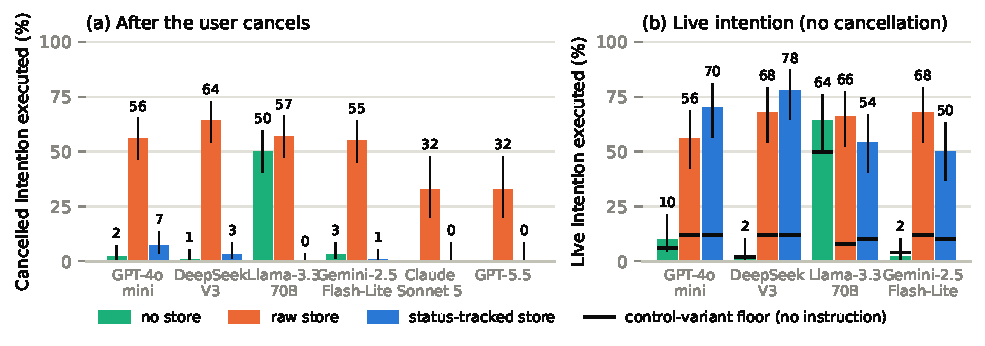
\includegraphics[width=\textwidth]{fig_main}
\caption{\textbf{(a)} How often each model executes an instruction \emph{after
the user cancelled it}, by memory regime (pooled early and late cancellation,
$n{=}100$; frontier models $n{=}40$). \textbf{(b)} How often the live
instruction is executed; the black tick is the control-twin floor, i.e.\ how
often the model switches the appliance off with no instruction at all.}
\label{fig:main}
\end{figure}

\begin{table}[t]
\centering\small
\caption{Development cell, pooled cancel arms ($n{=}100$; frontier $n{=}40$).
\eac{}: executed after cancellation (lower is better). \execm{}: live intention
executed. Floor: control twin. Tokens per episode in thousands.}
\label{tab:main}
\begin{tabular}{llrrrrr}
\toprule
Model & Regime & \eac{} & 95\% CI & \execm{} & Floor & tok/ep \\
\midrule
GPT-4o-mini & no store & \eacMiniNone{} & \eacCIMiniNone{} & \execMiniNone{} & \ctrlMiniNone{} & \tokMiniNone{}k \\
 & raw store & \eacMiniBank{} & \eacCIMiniBank{} & \execMiniBank{} & \ctrlMiniBank{} & \tokMiniBank{}k \\
 & status-tracked & \eacMiniSchedtwo{} & \eacCIMiniSchedtwo{} & \execMiniSchedtwo{} & \ctrlMiniSchedtwo{} & \tokMiniSchedtwo{}k \\
\midrule
DeepSeek-V3 & no store & \eacDeepseekNone{} & \eacCIDeepseekNone{} & \execDeepseekNone{} & \ctrlDeepseekNone{} & \tokDeepseekNone{}k \\
 & raw store & \eacDeepseekBank{} & \eacCIDeepseekBank{} & \execDeepseekBank{} & \ctrlDeepseekBank{} & \tokDeepseekBank{}k \\
 & status-tracked & \eacDeepseekSchedtwo{} & \eacCIDeepseekSchedtwo{} & \execDeepseekSchedtwo{} & \ctrlDeepseekSchedtwo{} & \tokDeepseekSchedtwo{}k \\
\midrule
Llama-3.3-70B & no store & \eacLlamaNone{} & \eacCILlamaNone{} & \execLlamaNone{} & \ctrlLlamaNone{} & \tokLlamaNone{}k \\
 & raw store & \eacLlamaBank{} & \eacCILlamaBank{} & \execLlamaBank{} & \ctrlLlamaBank{} & \tokLlamaBank{}k \\
 & status-tracked & \eacLlamaSchedtwo{} & \eacCILlamaSchedtwo{} & \execLlamaSchedtwo{} & \ctrlLlamaSchedtwo{} & \tokLlamaSchedtwo{}k \\
\midrule
Gemini-2.5-Flash-Lite & no store & \eacGeminiNone{} & \eacCIGeminiNone{} & \execGeminiNone{} & \ctrlGeminiNone{} & \tokGeminiNone{}k \\
 & raw store & \eacGeminiBank{} & \eacCIGeminiBank{} & \execGeminiBank{} & \ctrlGeminiBank{} & \tokGeminiBank{}k \\
 & status-tracked & \eacGeminiSchedtwo{} & \eacCIGeminiSchedtwo{} & \execGeminiSchedtwo{} & \ctrlGeminiSchedtwo{} & \tokGeminiSchedtwo{}k \\
\midrule
Claude Sonnet 5 & raw store & \eacSonnetBank{} & \eacCISonnetBank{} & -- & -- & \tokSonnetBank{}k \\
 & status-tracked & \eacSonnetSchedtwo{} & \eacCISonnetSchedtwo{} & -- & -- & \tokSonnetSchedtwo{}k \\
\midrule
GPT-5.5 & raw store & \eacGptffBank{} & \eacCIGptffBank{} & -- & -- & \tokGptffBank{}k \\
 & status-tracked & \eacGptffSchedtwo{} & \eacCIGptffSchedtwo{} & -- & -- & \tokGptffSchedtwo{}k \\
\bottomrule
\end{tabular}
\end{table}

Figure~\ref{fig:main} and Table~\ref{tab:main} give the main result.

\textbf{Without a store, nothing is executed.} Live-intention execution is at
the control floor for every model (\execMiniNone{}, \execDeepseekNone{},
\execGeminiNone{}): once the briefing leaves the window the instruction is gone.
This is the baseline that any memory pipeline improves on.

\textbf{The raw store restores execution and introduces violations.} Re-injecting
the briefing lifts \execm{} to \execPctMiniBank--\execPctDeepseekBank\%, but on
cancel twins the same models switch the appliance off after being told not to
in \eacPctMiniBank--\eacPctDeepseekBank\% of episodes. The two frontier models
are better but far from safe (\eacSonnetBank{} and \eacGptffBank{}). The
mechanism is visible in the traces: the store repeats ``turn it off'' every
step, the cancellation was one message that scrolled away, and the actor obeys
the text in front of it.

\textbf{Rewriting the entry fixes it on every model.} With the status-tracked
store, \eac{} falls to \eacMiniSchedtwo{} (GPT-4o-mini), \eacDeepseekSchedtwo{},
\eacLlamaSchedtwo{}, \eacGeminiSchedtwo{}, \eacSonnetSchedtwo{} and
\eacGptffSchedtwo{}. The store is information-matched to the raw store: same
chore line every step, same episode length (40 steps), same chores completed
(\choresMiniSchedtwo{} vs.\ \choresMiniBank{}), same tokens
(\tokMiniSchedtwo{}k vs.\ \tokMiniBank{}k) and comparable trigger exposure. Live
execution is not traded away (\execMiniSchedtwo{} vs.\ \execMiniBank{} on
GPT-4o-mini; \execDeepseekSchedtwo{} vs.\ \execDeepseekBank{} on DeepSeek).

\textbf{The control twin reads a prior as a prior.} Llama-3.3-70B switches the
appliance off in \ctrlLlamaBank{} control episodes with no instruction at all
(``turn it off for safety and energy efficiency''), so its \eacLlamaNone{} under
no store is not memory but habit. Its \execm{} gain from any store is nil
(execution is prior-driven), yet the \textsc{cancelled} entry suppresses even
the habit (\eacLlamaSchedtwo{}): execution is driven by the prior, revocation by
the instruction. Without the control twin this row would look like a bug.

\subsection{How the fix breaks}

\begin{figure}[t]
\centering
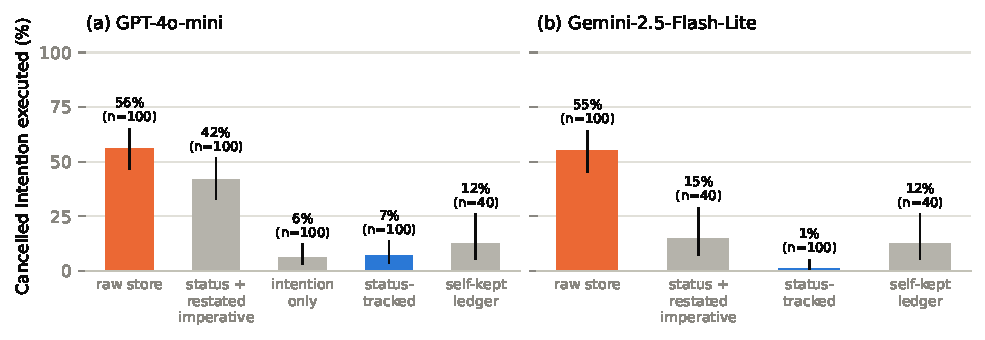
\includegraphics[width=\textwidth]{fig_ablation}
\caption{Execution after cancellation under five representations of the same
intention (development cell). The two anchor regimes from Fig.~\ref{fig:main}
are coloured; the three variants are grey.}
\label{fig:ablation}
\end{figure}

Figure~\ref{fig:ablation} varies only the representation.

\textbf{Restating the imperative undoes the revocation.} A cancellation entry
that still contains ``if you ever SEE the $X$ ON, turn it off'' after its
\textsc{cancelled} tag yields \eacMiniSchedone{} on GPT-4o-mini
($p=\pSchedoneSchedtwoMini$ vs.\ the rewritten entry) and is statistically
indistinguishable from having no revocation bookkeeping at all
($p=\pBankSchedoneMini$ vs.\ the raw store). On Gemini the same variant gives
\eacGeminiSchedone{} ($p=\pSchedoneSchedtwoGemini$). Small models read the
imperative, not the tag.

\textbf{Dropping the chore line makes agents quit early.} The intention-only
variant keeps violations low (\eacMiniSched{}) but agents complete
\choresMiniSched{} chores instead of \choresMiniSchedtwo{} and say ``done'' by
step 20: the chore list scrolled out of the window. Its low \eac{} is partly a
matter of never being around when the trigger fires, which is why the
information-matched status-tracked store is the regime we report.

\textbf{A self-kept ledger is compliant but forgetful.} When the model maintains
its own bank, violations stay low (\eacMiniRwim{} on GPT-4o-mini,
\eacGeminiRwim{} on Gemini) but live execution collapses to \execMiniRwim{} and
\execGeminiRwim{}; noticing is intact (\noticeMiniRwim\%) while execution given
noticing falls to \execSeenMiniRwim\%. The memory agent's notes show why: it
files chores as intentions, fires on the wrong conditions, and is silent when
the real trigger is on. The gap between this regime and the oracle-bookkeeping
ceiling is the concrete target \bench{} exposes.

\subsection{Robustness}

\begin{figure}[t]
\centering
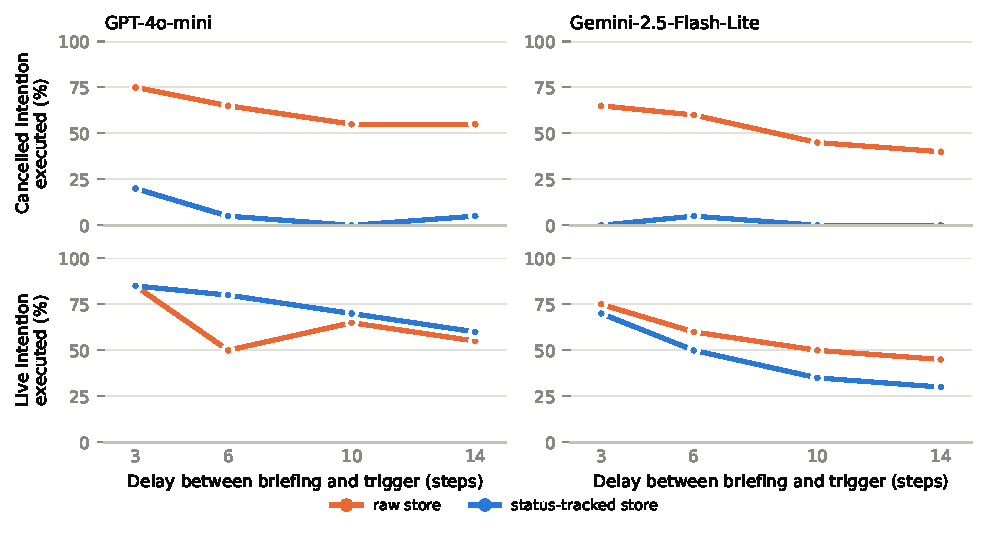
\includegraphics[width=\textwidth]{fig_delay}
\caption{Delay between briefing and trigger. Top: execution after cancellation
(early-cancel twins, $n{=}20$ per point; delay 6 uses the first 20 seeds of the
main cell). Bottom: live execution.}
\label{fig:delay}
\end{figure}

\textbf{Delay.} Figure~\ref{fig:delay} varies the delay between briefing and
trigger from 3 to 14 steps on two models. Raw-store violations stay between 40
and 75\% at every delay; status-tracked violations stay at or near zero; live
execution is matched between the two regimes at every point. The effect is not
an artefact of one window length.

\begin{table}[t]
\centering\small
\caption{Held-out kitchens (test split, early-cancel twins and live twins,
$n{=}20$ per cell). Raw store $\to$ status-tracked.}
\label{tab:heldout}
\resizebox{\textwidth}{!}{%
\begin{tabular}{lcccccc}
\toprule
 & \multicolumn{3}{c}{\eac{} (raw $\to$ status)} & \multicolumn{3}{c}{\execm{} (raw $\to$ status)} \\
Model & FP2 & FP3 & FP4 & FP2 & FP3 & FP4 \\
\midrule
GPT-4o-mini & \hoMiniTwoBank$\to$\hoMiniTwoSchedtwo & \hoMiniThreeBank$\to$\hoMiniThreeSchedtwo & \hoMiniFourBank$\to$\hoMiniFourSchedtwo & \hoExecMiniTwoBank$\to$\hoExecMiniTwoSchedtwo & \hoExecMiniThreeBank$\to$\hoExecMiniThreeSchedtwo & \hoExecMiniFourBank$\to$\hoExecMiniFourSchedtwo \\
Gemini-2.5-FL & \hoGeminiTwoBank$\to$\hoGeminiTwoSchedtwo & \hoGeminiThreeBank$\to$\hoGeminiThreeSchedtwo & \hoGeminiFourBank$\to$\hoGeminiFourSchedtwo & \hoExecGeminiTwoBank$\to$\hoExecGeminiTwoSchedtwo & \hoExecGeminiThreeBank$\to$\hoExecGeminiThreeSchedtwo & \hoExecGeminiFourBank$\to$\hoExecGeminiFourSchedtwo \\
\bottomrule
\end{tabular}}
\end{table}

\textbf{Held-out kitchens.} Table~\ref{tab:heldout} repeats the comparison in
three unseen kitchens with different layouts and appliances. The pattern holds
in every cell. GPT-4o-mini's \hoMiniFourSchedtwo{} in FloorPlan4 are all
faucet-triggered and cite the appliance state (``the faucet is on and I need to
turn it off'') with the \textsc{cancelled} entry present---a prior in the sense
of the control twin, and absent on Gemini (\hoGeminiFourSchedtwo{}).

\textbf{Pixels.} Replacing the symbolic observation with a 320$\times$240 frame
(the history then carries only inventory and messages) turns the task into a
perception problem for the two cheap vision models we tried: with the trigger
lit and in view, GPT-4o-mini executes \rgbExecSeenMiniBank{} (raw) and
\rgbExecSeenMiniSchedtwo{} (status-tracked) times, Gemini
\rgbExecSeenGeminiBank{} and \rgbExecSeenGeminiSchedtwo{}. The appliance's
state is not legible to these models at this resolution, so no memory regime can
be discriminated on the pixel tier; we report it as a negative result and keep
the symbolic tier, which isolates memory from perception by construction.

\section{Limitations}

The status-tracked store reads the cancellation time from ground truth; it
bounds what correct bookkeeping achieves and is not a deployable method (the
self-kept ledger is the non-privileged counterpart). Development cells use one
intention per episode; the multi-intention cells of the suite were run only
with scripted agents. The Habitat tier has no LLM results. All actors are API
models with a symbolic observation interface; end-to-end vision-language-action
policies and pixel-level perception with frontier vision models are future work.
Sample sizes are 50 per variant (20 for frontier models), adequate for the
effect sizes reported but not for small ones.

\section{Conclusion}

\bench{} grades the full lifecycle of a deferred instruction---given, triggered
out of view, executed, and revoked---from world state, with twin episodes that
attribute every difference to the instruction. Across six model families the
failure that matters is not forgetting an instruction but forgetting its
cancellation, and it is a property of how the intention is stored, not of the
model: rewriting a status-tracked entry removes it everywhere, restating the
imperative brings it back, and a small model keeping its own ledger stays safe
only by doing less. Bookkeeping of intentions is a measurable target, and this
benchmark measures it.

\subsubsection*{AI use statement}
Language-model assistance was used for code, experiment orchestration and
editing. All experimental design decisions, analyses and claims were made and
verified by the authors.

\bibliography{refs}
\bibliographystyle{iclr2027_conference}

\end{document}
